\chapter{Конструкторская часть}
В этом разделе будут представлено описание используемых типов данных, а также схемы алгоритмов поиска в словаре.

\section{Требования к программному обеспечению}

К программе предъявлены ряд требований:

\begin{itemize}[label=---]
	\item иметь интерфейс ввода вопроса;
	\item работа с словарями и массивами;
	\item работа со строками.
\end{itemize}

\section{Описание используемых типов данных}
При реализации алгоритмов будут использованы следующие типы данных:
\begin{enumerate}[label=\arabic*)]
	\item словарь --- встроенный тип dict \cite{pythondict} в Python\cite{pythonlang} будет использован в созданном классе Dictionary;
	\item массив ключей --- встроенный тип list \cite{pythonlist} в Python\cite{pythonlang};
	\item длина массива/словаря --- целое число int.
\end{enumerate}

\section{Разработка алгоритмов}

На рисунке \ref{fig:full_comb} представлена схема алгоритма поиска в словаре полным перебором.

\begin{figure}[h]
	\centering
	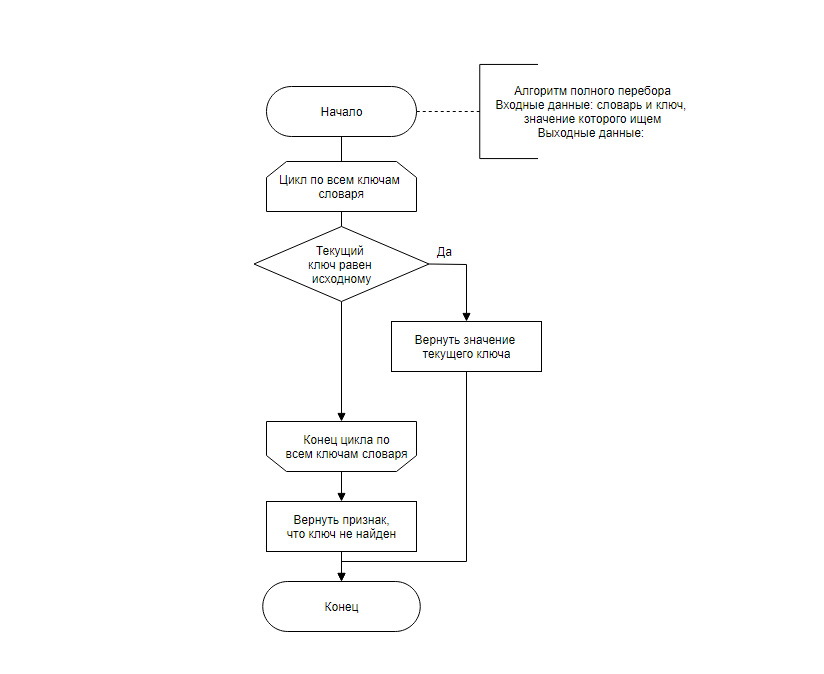
\includegraphics[width=0.85\textwidth]{img/full_comb.png}
	\caption{Схема алгоритма поиска в словаре полным перебором}
	\label{fig:full_comb}
\end{figure}

\section{Вывод}
В данном разделе была построена схема алгоритма, рассматриваемого в лабораторной работе, были описаны классы эквивалентности для тестирования, структура программы.
